\documentclass{article}
\usepackage{graphicx}
\usepackage{amssymb}
\usepackage{amsmath}
\usepackage{tikz}
\usepackage{url}
\usepackage{color}
\usepackage{savetrees}
% \usetikzlibrary{shapes}


\linespread{1.5}
\setlength{\parindent}{0pt}
\setlength{\parskip}{1.9ex plus 0.5ex minus 0.2ex}

% \linespread{1.4}

\title{CSE613\\Parallel Programming -- Homework-1}

\author{Dhruv Matani (108267786) \& Gaurav Menghani (108266803)}

\renewcommand{\thesubsection}{\thesection\ (\alph{subsection})}

\begin{document}
\maketitle

\clearpage

\tableofcontents

\clearpage

\section{Pairwise Sequence Alignment with Affine Gap Costs}

Compiling all the programs:
\begin{verbatim}
$ cd Prob-1
$ make
\end{verbatim}

\subsection{Serial algorithm}

Please check archive for the code

Running the code:
\begin{verbatim}
$ a/a.out < input_file_path
\end{verbatim}

\subsection{Parallelized algorithm by parallelizing the computation of the diagonal}

Running the code:
\begin{verbatim}
$ b/a.out [string size in bytes in the input file (this is a power of 2)] 1 < input_file_path
\end{verbatim}

\textit{Analysis of the resulting parallelism:} $T_{\infty} = \log{1} + \log{2} + \log{3} + \log{4} + \ldots{} + \log{n}$

$\Rightarrow T_{\infty} = \log{n!}$

$\Rightarrow T_{\infty} = n\log{n}$

$\therefore$ Parallelism = $\dfrac{n^2}{n\log{n}} = \dfrac{n}{\log{n}}$

\subsection{Parallel Divide \& Conquer algorithm}

Running the code:
\begin{verbatim}
$ c/a.out [base case size (this is a power of 2 - default: 16)] < input_file_path
\end{verbatim}

The best running time we got was for a base case of a block of size $32 \times 32$ elements.

\subsection{Parallelism and space usage of the Parallel Divide \& Conquer algorithm}

$T_{\infty}(n) = 3T_{\infty}(\frac{n}{2}) + O(1)$

$\Rightarrow T_{\infty}(n) = n^{\log_2{3}} = n^{1.58}$

$\therefore$ Parallelism = $\dfrac{n^2}{n^{1.58}} = n^{0.42}$

Space usage is $O(n^2)$.

\subsection{Boundary Generation parallel LCS algorithm}

The best running time we got was for a base case of a block of size $FIXME$ elements.

Running the code:
\begin{verbatim}
$ e/a.out [base case size (this is a power of 2 - default: 16)] < input_file_path
\end{verbatim}

\subsection{Parallelism and space usage of the Boundary Generation parallel LCS algorithm}

$T_{\infty}(n) = Q(\frac{n}{q})\log{1} + Q(\frac{n}{q})\log{2} + Q(\frac{n}{q})\log{3} + Q(\frac{n}{q})\log{4} + \ldots{} + Q(\frac{n}{q})\log{\frac{n}{q}}$

But, $Q(m) = m^{\log_2{3}}$, which is the time to solve a problem of size $m$ using the Divide \& Conquer algorithm.

$\therefore T_{\infty}(n) = Q(\dfrac{n}{q})q\log{(q+1)}$

$\Rightarrow T_{\infty}(n) = q\log{(q+1)}\left(\dfrac{n}{q}\right)^{\log_2{3}}$

$\therefore$ Parallelism = $\dfrac{n^2}{q\log{(q+1)}(\frac{n}{q})^{\log_2{3}}} = \dfrac{n^2}{q\log{(q+1)}(\frac{n}{q})^{\log_2{3}}}$

Space usage is $O(n^2)$.

\subsection{Limit on $n$ and Cilkview scalability plots}

The limit on $n$ we experimentally determined happens to be ${n'}_{max} = 32768$.

\begin{figure}
  \begin{center}
    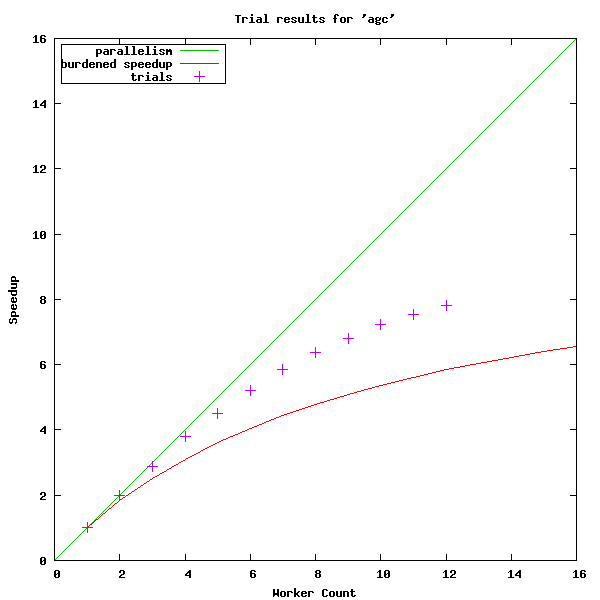
\includegraphics[width=4in]{images/agc-partc.png}
    \caption{Cilkview plot for part(c) - Divide \& Conquer solution}
    \label{fig:cilkview_c}
  \end{center}
\end {figure}

\begin{figure}
  \begin{center}
    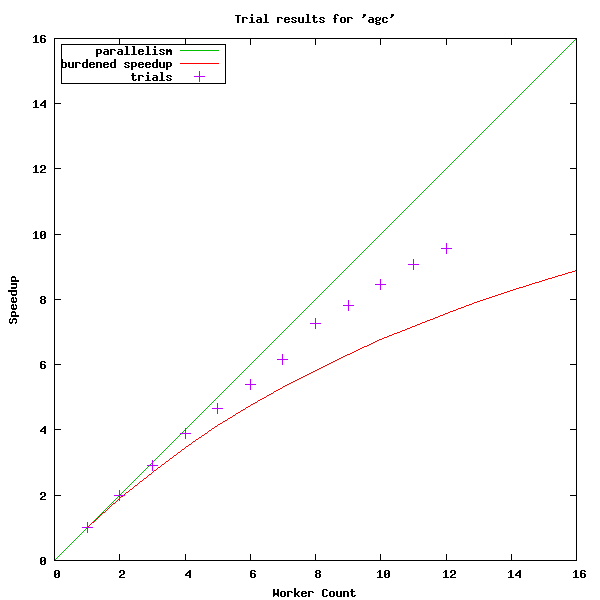
\includegraphics[width=4in]{images/agc-parte.png}
    \caption{Cilkview plot for part(e) - Cache Efficient blocking-based diagonal solution}
    \label{fig:cilkview_e}
  \end{center}
\end {figure}


\subsection{Limit on $n$, \texttt{PAPI} for number of L1 cache misses for the parallel \& serial implementation}
The number of L1 and L2 misses for part (a) are as follows:\\
L1 Misses: 224395558\\
L2 Misses: 7937023\\

The number of L1 and L2 misses for part (c) are as follows:\\
L1 Misses: 692573496\\
L2 Misses: 364397656\\
\\
There are more cache misses in part (c) because, there is no data locality
as compared to part (a), which has better data locality.

\clearpage

\section{Pairwise Alignment for Highly Uneven Sequence Lengths}

\subsection{Parallelism of diagonal parallel solution for highly uneven sequences}

If $m \ll n$ and $m \ll p$, then the parallel running time of the earlier algorithm on the uneven sequences would be:

$T_{\infty} = O(n\log{m})$

The serial running time, $T_1 = O(nm)$

$\therefore$ Parallelism $= \dfrac{nm}{n\log{m}} = \dfrac{m}{\log{m}}$

\subsection{Optimized Parallel Algorithm for solving highly uneven sequences}

The algorithm to compute the edit distance for highly uneven sequences is described below:

\begin{enumerate}

\item We lay out the matrix so that it has $m$ rows and $n$ columns.

\item We first compute (for the first row), the value in each cell
  depending on the corresponding cell in the previous row and the
  diagonally opposite cell in the previous row. We do NOT us the value
  in the previous cell in the SAME row. Work: $O(n)$, depth: $O(\log{n})$

\item Now, we compute costs for each cell assuming that an INSERT GAP
  started at that cell. This can be done using a parallel for-loop
  with work $O(n)$ and depth $O(\log{n})$.

\item Now, for each cell (at index $k$), we take the minimum value in
  each cell before it and subtract from that value the number
  $(n-k)$. This will give us the value in that cell. This can be done
  using $O(n)$ work, and $O(\log{n})$ depth since we can pre-compute
  the value for each range from $[0 \ldots{} k]$.

\item We do this for each of the $m$ rows in the matrix.

\end{enumerate}

$T_1 = O(mn)$

$T_{\infty} = O(m\log{n})$

$\therefore$ Parallelism $= \dfrac{mn}{m\log{n}} = \dfrac{n}{\log{n}} \gg \dfrac{m}{\log{m}}$ for $m \ll n$.

\subsection{Extending the algorithm to solve Part-1}

The algorithm can easily be extended to solve Part-1 since we can add
the value $g_i$ every time we start a gap at a certain index.

$T_1 = O(n^2)$

$T_{\infty} = O(n\log{n})$

$\therefore$ Parallelism $= \dfrac{n^2}{n\log{n}} = \dfrac{n}{\log{n}}$.

We get the same parallelism as Part-1 (f) if we set $q = n$.

\clearpage

\section{Randomized Parallel Quicksort with Looping}

\subsection{Upper bound on recursion depth of \texttt{PAR-RANDOMIZED-LOOPING-QUICKSORT}}

We know that the routine \texttt{PAR-PARTITION} randomly splits its
input, but the routine \texttt{PAR-RANDOMIZED-LOOPING-QUICKSORT}
doesn't continue unless the split is at least between
$\frac{1}{4}^{th}$ \& $\frac{3}{4}^{th}$.

What this means is that the upper bound on the depth of
\texttt{PAR-RANDOMIZED-LOOPING-QUICKSORT} is determined by the
following recurrence:

$T(n) = T(\frac{3n}{4}) + 1$

$\Rightarrow T(n) = \log_{4/3}{n}$

$\Rightarrow T(n) = \dfrac{\ln{n}}{\ln{4/3}}$

$\Rightarrow T(n) = 3.48\ln{n} < 8\ln{n}$

\subsection{Proof of expected depth and work}

Since \texttt{PAR-PARTITION} chooses a pivot at random, the
probability of choosing a \textit{good} pivot (i.e. a pivot that
splits the input into at most $\frac{1}{4}^{th}$ \&
$\frac{3}{4}^{th}$) is $\frac{1}{2}$.

Hence, it is \textit{expected} that only half the times will
\texttt{PAR-PARTITION} choose a bad pivot. The other half times, it
will choose a good pivot. Therefore, the expected number of times
\texttt{PAR-PARTITION} will be called before it chooses a
\textit{good} pivot is:

$E[number\ of\ calls] = \frac{1}{2} \times 1 + \frac{1}{2}^2 \times 2 +
\frac{1}{2}^3 \times 3 + \frac{1}{2}^4 \times 4 + \ldots$

$\Rightarrow E[number\ of\ calls] = 2$

Therefore, \texttt{PAR-PARTITION} splits its input into a constant
fraction at most every other time it is called (in an expected
sense). This makes the depth of
\texttt{PAR-RANDOMIZED-LOOPING-QUICKSORT} $O(\log^{3}{n})$, and the
work done $O(n\log{n})$.

\subsection{Tracking an Element}

We know that the depth of \texttt{PAR-RANDOMIZED-LOOPING-QUICKSORT}
(excluding that of \texttt{PAR-PARTITION}) is $< 4\ln{n}$.

The expected number of times we call \texttt{PAR-PARTITION} per call
of \texttt{PAR-RANDOMIZED-LOOPING-QUICKSORT} is 2.

Hence, the expected number of times an element $v$ of the array
features in an array passed to \texttt{PAR-PARTITION} is $R_v =
8\ln{n}$.

We shall now use Chernoff Bounds. $E[x] = 8\ln{n}$. We need to show
that $R_v < 32\ln{n}$ with high probability.

$\therefore Pr(X > (1 + \delta)E[X]) \le 
\left(\dfrac{e^\delta}{(1+\delta)^{(1+\delta)}}\right)^{E[X]}$

Here, $(1 + \delta)E[X] = 32\ln{n}$

$\therefore (1+\delta)8\ln{n} = 32\ln{n}$

$\Rightarrow (1+\delta) = 4$

$\Rightarrow \delta = 3$

$\therefore Pr(X > (1 + \delta)E[X]) \le 
\left(\dfrac{e^3}{4^4}\right)^{8\ln{n}}$

$\le \left(\dfrac{1}{12.75}\right)^{8\ln{n}}$

$\le \left(\dfrac{1}{698363412.02}\right)^{\ln{n}}$

$\le \left(\dfrac{1}{n}\right)^{\ln{698363412.02}}$

$\le \left(\dfrac{1}{n}\right)^{20.36}$

$\le \dfrac{1}{n^{20.36}} \le \dfrac{1}{n^{2}}$

\subsection{Proof of depth and work with high probability}

In part $(3.3)$ above, we showed that a randomly chosen element
doesn't feature is more than $32\ln{n}$ calls to
\texttt{PAR-PARTITION} with high probability.

Hence, the depth and work of \texttt{PAR-PARTITION} is $O(\ln^2{n})$
and $O(n)$ respectively with high probability.

This makes the depth and work of
\texttt{PAR-RANDOMIZED-LOOPING-QUICKSORT} $O(\ln^3{n})$ and
$O(n\ln{n})$ respectively with high probability.


\end{document}
